\chapter{Solution design}
\label {solutiondesign}

The executor contains of two parts: the main node and the agents. The agent runs on the created VMs, manages starting / updating / removing of the docker containers, executing of the distributed plan and provides information about current allocation and docker inspect output. The main node manages executing of the monolithic plan, and also provides current allocation and docker inspect output. The main node provides the allocation by sending requests to each known agent and aggregating answers.

\section{Problems}
\subsection{Bin packing problem}
  The monolithic approach given current allocation and the monolithic plan (resource demand for each tier) should do creation / deletion of VMs and allocation containers on them. This problem is similar to well-known Bin packing problem. A VM for us is a bin and a container is an object which we need to pack in the bin. The container has two dimensions: CPU cores and RAM, so this is 2D bin packing problem. The main difference to bin packing problem is that we have initial allocation (initial packing) and we should not only minimize number of bins used, but also number of movements required to reach the final allocation from the initial one.
  
  The linear optimisation problem was formulated to solve this 2d bin packing problem:
  
\begin{equation*}
\text{minimize } \displaystyle\sum\limits_{i \in I}^{}\sum\limits_{j \in J}^{} (w_{0ij} \alpha_{0ij} + w_{1ij} \alpha_{1ij}) + \sum\limits_{i \in I}^{} (w_{2i} \beta_{0i} + w_{3i} \beta_{1i})
\end{equation*}
\begin{equation*}
\begin{array}{ll@{}ll}
\text{subject to} & & &\\
\text{(1)}           & \displaystyle\sum\limits_{j \in J}^{} x_{ij} \leq m_{0i} \beta_{0i}  & & \forall i \in I\\
\text{(2)}           & \displaystyle\sum\limits_{j \in J}^{} y_{ij} \leq m_{1i} \beta_{0i} & & \forall i \in I\\
\text{(3)}           & \displaystyle  x_{ij} \leq m_{0i} \alpha_{ij} & & \forall i \in I, j \in J\\
\text{(4)}           & \displaystyle y_{ij} \leq m_{1i} \alpha_{ij} & & \forall i \in I, j \in J\\
\text{(5)}           & \displaystyle\sum\limits_{i \in I}^{} x_{ij} = d_{0j} & & \forall j \in J\\
\text{(6)}           & \displaystyle\sum\limits_{i \in I}^{} y_{ij} = d_{1j} & & \forall j \in J\\
\text{(7)}           & \displaystyle m_{1i} x_{ij} \geq y_{ij} & & \forall i \in I, j \in J\\
\text{(8)}           & \displaystyle m_{0i} y_{ij} \geq x_{ij} & & \forall i \in I, j \in J\\
\text{(9)}           & \displaystyle \alpha_{0ij} + \alpha_{1ij} = 1 & & \forall i \in I, j \in J\\
\text{(10)}          & \displaystyle \beta_{0i} + \beta_{1i} = 1 & & \forall i \in I\\
                     & \alpha_{0ij} \in \{0, 1\}  & & \forall i \in I, j \in J\\
                     & \alpha_{1ij} \in \{0, 1\}  & & \forall i \in I, j \in J\\
                     & \beta_{0i} \in \{0, 1\}  & & \forall i \in I\\
                     & \beta_{1i} \in \{0, 1\}  & & \forall i \in I\\
                     & x_{ij} \in \mathbb{Z}  & x_{ij} \geq 0 & \forall i \in I, j \in J\\
                     & y_{ij} \in \mathbb{Z}  & y_{ij} \geq 0 & \forall i \in I, j \in J\\
\end{array}
\end{equation*}
where \\
\indent $I$ is the set of VMs,\\
\indent $J$ is the set of Tiers,
\begin{sloppypar} $\alpha_{0ij}$ is "tier\_is\_used" binary variable that is true if we allocate container for tier[j] on VM[i],
\indent $\alpha_{1ij}$ is "tier\_is\_idle" binary variable that is true only if $\alpha_{0ij}$ is false, the equation (9) links them together,
\indent $\beta_{0i}$ is "vm\_is\_used" binary variable that is true if we allocate any container for any tier on VM[i],
\indent $\beta_{1i}$ is "vm\_is\_idle" binary variable that is true only if $\beta_{0i}$ is false, the equation (10) links them together,
\indent $x_{ij}$ is "cpu\_usage" variable: the number of CPU cores that tier[j] uses on VM[i],
\indent $y_{ij}$ is "mem\_usage" variable: "the number of RAM units (1 unit = 512Mb) that tier[j] uses on VM[i],
\indent (1) is CPU availability constraint and constraint for activation of "vm\_is\_used" variable, constant $m_{0i}$ is the number of CPU cores on VM[i] (maximum allowed value for $x_{ij}$),
\indent (2) is the same as (1), but for the RAM units, constant $m_{1i}$ is the number of RAM units on VM[i] (maximum allowed value for $y_{ij}$) 
\indent (3) and (4) are activation of $\alpha_{ij}$ constraints similar to (1) and (2). (3) is for CPU cores, (4) is for RAM units,
\indent (6) is the RAM units demand equation, where $d_{1j}$ is the RAM units demand from the plan for the tier[j],
\indent (5) is the same as (4), but for the CPU cores, $d_{0j}$ is the CPU cores demand from the plan for the tier[j],
\indent (7) says that if tier[j] uses some RAM on VM[i], then it must use some CPU cores,
\indent (8) is the same as constraint (7), but other way round: if tier[j] uses some CPU cores on VM[i], then it must use some RAM units.
\end{sloppypar}

This formulation of the problem requires us to know the number of VMs beforehand, which we do not know. So the upper bound number of VMs is calculated and provided to the ILP solver. VMs that are used in the initial allocation are already created, but there are also VMs that are empty and are only going to be created if there will be some container on it.

Considering the initial allocation is done by constants $w_{0ij}, w_{1ij}, w_{2i}, w_{3i}$.
Where $w_{0ij}$ is the constant for using tier[j] on VM[i], so knowing initial allocation we can set this constant to the cost of the container creation if there is no tier[j] on VM[i] in the initial allocation, and the cost of the container update if there is tier[j] on VM[i] in the initial allocation. Here is a pitfall that if in the initial allocation container was used on the VM, and we use it in the new allocation, we can not differentiate if the value of CPU cores and RAM units used has changed (we need to run container update command) or is not changed (we need do nothing).

The weight constant $w_{1ij}$ is the cost of removing container of the tier[j] from the VM[i], this weight should be 0 if the tier[j] was not on the VM[i] in the initial allocation.

The weight $w_{2i}$ is the cost of VM[i] creation. if VM[i] is already used in the initial allocation this constant is 0.

The weight $w_{3i}$ is the cost of using the VM[i]. This cost is 0, if 
the VM is not created yet, and it was not used in the initial allocation.

Considering NFR-2, the weights for actions should follow these rules: 
\begin{enumerate}
    \item container delete \textless{ } container update \textless{ } container create
    \item VM delete \textless{ } VM use \textless{ } VM create
    \item VM delete + container delete  + container create \textless{ } \\ VM use + container update
\end{enumerate}

 \begin{sloppypar} The rule number 3 is introduced, because it is possible a situation when for example we can remove some VM[p], this VM had in the initial allocation 1 container. The weight of vm\_usage=30, the weight of vm\_deletion=25, the weight of container\_update=10, the weight of container\_deletion=5, the weight of container\_create=15. So to continue to use this VM the objective function will have $vm\_usage + container\_update=30 + 10 = 40$, and to remove this container in the worst case we need to create container in another place: $vm\_deletion + container\_deletion + container\_create = 25 + 5 + 15 = 45$. So ILP minimizing the objective function will choose not to remove the VM[p], but keep it. This is against our requirement NFR-0 and we want to keep the minimum number of VMs possible. 
 \end{sloppypar}
 
 Also NFR-2 requires weight of "container use" be less than "container update", but I could not found the easy way to differentiate them in ILP. As we have initial allocation as constants, for example $c_{ij}$ is CPU cores used by container[j] on VM[i] and $m_{ij}$ is the same for RAM units. The new allocation in the ILP are variables $x_{ij}$ and $y_{ij}$ for CPU cores and RAM units accordingly. So to differentiate "container use" from "container update", we need either $x_{ij} + y_{ij} \neq c_{ij} + m_{ij}$ or $abs(x_{ij} + y_{ij} - c_{ij} - m_{ij}) > 0$ or some "if" constraint that all makes our ILP non linear. The effective workaround to solve this issue is considered out of scope of this paper.

\subsection{Scalability}
The tier can be scalable or not. The not scalable tier can have only 1 or 0 containers. If the tier is absent in the plan, it will have 0 containers, otherwise it will be 1, whilst the scalable tier can have any number of containers $\geq 0$ allocated on different VMs. In the ILP formulation not scalable containers are not considered, so the current workaround is too 

\subsection{Limitation of the ILP formulation}
This ILP formulation has some limitations:
\begin{enumerate}
    \item This formulation of the problem requires us to know the number of VMs beforehand, which we do not know. But we can make upper-bound estimation.
    \item This formulation does not differentiate between "container update" and "container use" (do nothing with container). 
    \item Weights should be chosen wisely to satisfy NFR-0.
    \item Bin packing problem is NP-hard
    \item We have 1 optimal solution and can not choose between several different solutions
\end{enumerate}

\subsection{Hooks}
Hooks are scripts that trigger on the tier / container scaling. The goal is to adjust the application's configuration after the allocation is changed.

We tried to extract and describe use cases of adjusting required:
\begin{enumerate}
    \item Jboss needs to adapt the number of threads considering the number of CPU allocated.
    \item LoadBalancer needs to be provided with the list of Jboss containers and resources allocated to adapt it weights.
    \item Jboss needs to be provided with the DB address on container creation / change.
\end{enumerate}

The adjustment 1 should be run for the container after it is created or updated. We call this adjustment "scale-hook" or "on\_node\_scale" hook. The script should be provided with 4 arguments: previous CPU cores allocated, previous RAM memory units allocated, and new CPU cores and RAM memory units allocated.

In the 2nd adjustment   the LoadBalancer tier depends on the Jboss tier. So the dependencies should be specified. Also the dependent node (LoadBalancer) should wait until all the containers of the dependee are processed (JBOSS). After that the adjustment script should be run on all the containers of the dependent node (LoadBalancer). We call this adjustment "tier-hook" or "on\_dependency\_scale" hook.

The 3d adjustment should be run only on the container start. To simpliy the first version of the application we decided not to implement this adjustment for the dependecy 1-to-n. Only for the dependencies n-to-1 and 1-to-1 after the dependee tier is processed, the ip of the dependee tier is provided to the dependent node on the creation (parameter "add-host"). 

This creates some limitations: the dependee container should be processed before dependent containers. For example, if the first plan will have only dependent containers, in the next plan it will be added dependee container, and in the last plan the dependence between them will be specified, then "add-host" feature will not be propagated and the dependee containers will not know about the dependant one.

Similar problem if we decided to remove the not-scalable tier from the plan, the dependee containers will have not valid "add-host" link and even if later we put the "not-scalable" tier back to the plan, it will have another IP address.

So considering these limitations we suggest one of the two workarounds.

The first is to manage the DB dependencies out of the topology and provide the IP address in the topology as "docker parameter".

The second is just use docker "add-host" feature as it. So if the dependent container is removed, or the dependency is added, the user should be aware that "add-host" will not be specified.

\subsection{Dependencies}
Considering the requirement FR-9 only 1-to-1, 1-to-n and n-to-1 dependencies are supported. The dependencies between scalable tiers are not supported. The dependencies are only used to manager tier-hooks and . 
The flow for container allocation and hooks execution should be:
\begin{enumerate}
    \item get tiers dependency graph (G)
    \item get set of Tiers without outgoing dependencies (T)
    \item run container create / update / delete for each tier in T
    \item run scale hooks if needed for each tier container in T
    \item run tier hooks if needed for each tier container in T
    \item remove T from G
    \item if G is not empty go to 2
\end{enumerate}

\section{Approaches}
Besides the ILP approach to solve container allocation problem discussed above it was also tried another approache: Constraint Satisfaction Problem.

\subsection{Constraint Satisfaction Problem}

CSP is defined as a triple \textless X, D, C\textgreater, where $X$ is a set of variables, $D$ is a set of the respective domains of values, $C$ is a set of constraints.

In our context we have 2 matrices of variables as $X$: \\
$x_{ij}$ is a matrix that specify how many CPU is used by Tier[j] on VM[i],\\
$y_{ij}$ is a matrix that specify how many RAM units are used by Tier[j] on VM[i].

The domain $D$ for us is all possible values of CPU cores and RAM units. For example if we have AWS t2.medium with 2 CPU cores and 8 RAM units, we have: \\
$d_{0ij}$ is $\{0, 1, 2\}$ for CPU cores,\\
$d_{1ij}$ is $\{0, 1, 2, 3, 4, 5, 6, 7, 8\}$ for RAM mem units.

For a set of constraints $C$ we should consider similar to ILP:
\begin{itemize}
    \item availability constraints on each VM for CPU cores and for RAM mem units
    \item demand constraint considering the plan
    \item 0 CPU cores with RAM \textgreater{} 0 or other way round
\end{itemize}

\subsection{Limitation of the CSP}
This CSP formulation has also some limitations:
\begin{enumerate}
    \item Comparing to ILP, changing domain to continuous values may cause problems.
    \item The solution of the CSP is a list of different solutions, that can differ only by a permutation. We can have a factorial number of different solutions which we need to look to found the optimal one considering the initial allocation.
    \item The problem is NP-Hard and the complexity growth is much faster than the ILP.
\end{enumerate}

The CSP formulation has one insuperable problem that it does not scale. If we have 10 Tiers, 10 VMs, and 16 CPU cores and 64 RAM mem units, the CSP solution does not complete in appropriate time.

\section{Architecture}

\begin{figure}[ht]
  \centering
    \includegraphics[width=350px,natwidth=688,natheight=617]{./pictures/architecture}
    \caption{Architecture}
\end{figure}

The architecture consists of two main components: Executor Main Node and Executor Agent. The main node accepts a monolithic plan, orchestrates agents 
and has a whole picture of VMs allocated. The agent node can accept a distributed plan to execute, can run / start / stop docker containers, provides the allocation information and output of docker inspect command.

These executor nodes are "Execute" part of the autonomous system MAPE framework. The Monitor component measures different metrics of applications that are
running in the containers on the Executor agents, and provide this information to the Analyze component. The Plan component together with the Analyze component produce a new plan (a resource demand for tiers) which is sent to Executor.

\clearpage
\subsection{Components}
\begin{figure}[ht]
  \centering
    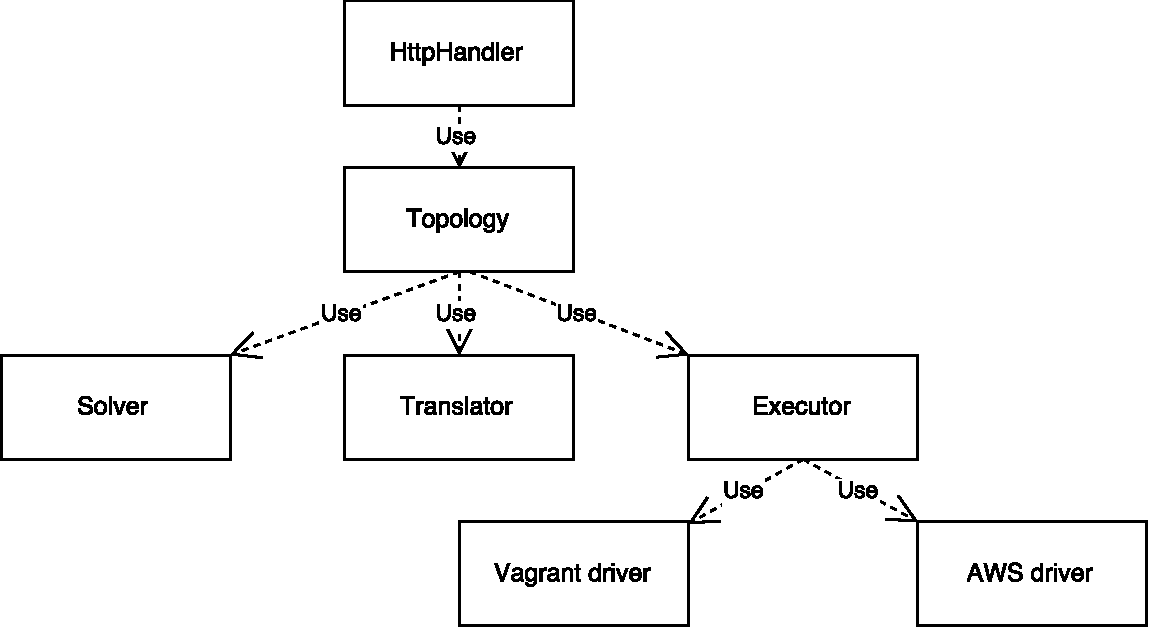
\includegraphics[width=350px,natwidth=553,natheight=303]{./pictures/main-classes}
    \caption{Executor main node classes}
\end{figure}

\begin{figure}[ht]
  \centering
    \includegraphics[height=150px,natwidth=113,natheight=203]{./pictures/agent-classes}
    \caption{Executor agent node classes}
\end{figure}